% report_toric_ideal.tex
% Report on toric ideal calculation task on Computer Algebra course.
% Vladimir Rutsky <altsysrq@gmail.com>
% 22.12.2009

\documentclass[a4paper,12pt]{article}

% Encoding support.
\usepackage{ucs}
\usepackage[utf8x]{inputenc}
\usepackage[T2A]{fontenc}
\usepackage[russian]{babel}

\usepackage{amsmath, amsthm, amssymb}

% Indenting first paragraph.
\usepackage{indentfirst}

%\usepackage{url}
\usepackage{hyperref}

\usepackage[final]{pdfpages}

% Spaces after commas.
\frenchspacing
% Minimal carrying number of characters,
\righthyphenmin=2

% From K.V.Voroncov Latex in samples, 2005.
\textheight=24cm   % text height
\textwidth=16cm    % text width.
\oddsidemargin=0pt % left side indention
\topmargin=-1.5cm  % top side indention.
\parindent=24pt    % paragraph indent
\parskip=0pt       % distance between paragraphs.
\tolerance=2000
%\flushbottom       % page height aligning
%\hoffset=0cm
%\pagestyle{empty}  % without numeration

\title{Отчет \\ Вычисление торических идеалов}
\author{Владимир Руцкий, 4057/2}

\newcommand{\commandquote}[1]{\textbf{#1}}

\begin{document}

% Title page.
\maketitle
% Content

\section{Постановка задачи}
Дана система уравнений вида:
\begin{align}
  y_1    & = x_1^{c_{11}} x_2^{c_{12}} x_3^{c_{13}} \cdots x_m^{c_{1m}} \notag\\
  y_2    & = x_1^{c_{21}} x_2^{c_{22}} x_3^{c_{23}} \cdots x_m^{c_{2m}} \label{eq-source}\\
         & \quad\quad\quad \vdots \notag\\ % TODO
  y_n    & = x_1^{c_{n1}} x_2^{c_{n2}} x_3^{c_{n3}} \cdots x_m^{c_{nm}} \notag
\end{align}

Или:
\begin{align}
   0 & = -y_1 + x_1^{c_{11}} x_2^{c_{12}} x_3^{c_{13}} \cdots x_m^{c_{1m}} \notag\\
   0 & = -y_2 + x_1^{c_{21}} x_2^{c_{22}} x_3^{c_{23}} \cdots x_m^{c_{2m}} \label{eq-source-reduced}\\
          & \quad\quad\quad\quad\quad \vdots \notag\\ % TODO
   0 & = -y_n + x_1^{c_{n1}} x_2^{c_{n2}} x_3^{c_{n3}} \cdots x_m^{c_{nm}} \notag
\end{align}

Эта система задаёт идеал $\mathfrak{a}$ в кольце многочленов $K[y_1, \ldots, y_n, x_1, \ldots, x_m]$.

Требуется найти подидеал $\mathfrak{a}' \subset \mathfrak{a}$, содержащий только переменные из $\{y_1, \ldots, y_n\}$.

\section{Выбранный метод решения}
Построим базис Грёбнера для $\mathfrak{a}$ с помощью алгоритма Бухбергера с таким упорядочением мономов, 
чтобы в первую очередь из системы \eqref{eq-source-reduced} были редуцированы 
мономы из $\{x_1, \ldots, x_m\}$.
Таким упорядочением является лексикографический порядок, 
в котором $\forall i, j \quad x_i > y_j$.

\section{Дополнительные исследования}
Система \eqref{eq-source} задаёт гомоморфизм $\Theta$ между двумя полями многочленов $K_1$ и $K_2$:
$$\Theta: K_1[y_1, \ldots, y_n] \rightarrow K_2[x_1, \ldots, x_m].$$

Подидеал $\mathfrak{a}'$ в такой интерпретации задаёт $\textrm{ker}\ \Theta$, т.\,к. $\forall v \in \mathfrak{a}' \quad \Theta(v) = 0$.

\section{Реализация решения}
Задача была решена в системе компьютерной алгебры 
Maxima\footnote{\url{http://maxima.sourceforge.net/}~--- Maxima, a Computer Algebra System}, 
с использованием пакета grobner.

Число переменных было фиксировано на значениях $n = 7$, $m = 3$.
Матрица степеней $c(n, m)$ была заполнена произвольными целыми степенями из диапазона $[0, 4]$,
её можно найти в приложении с исходным кодом и результатами решения.

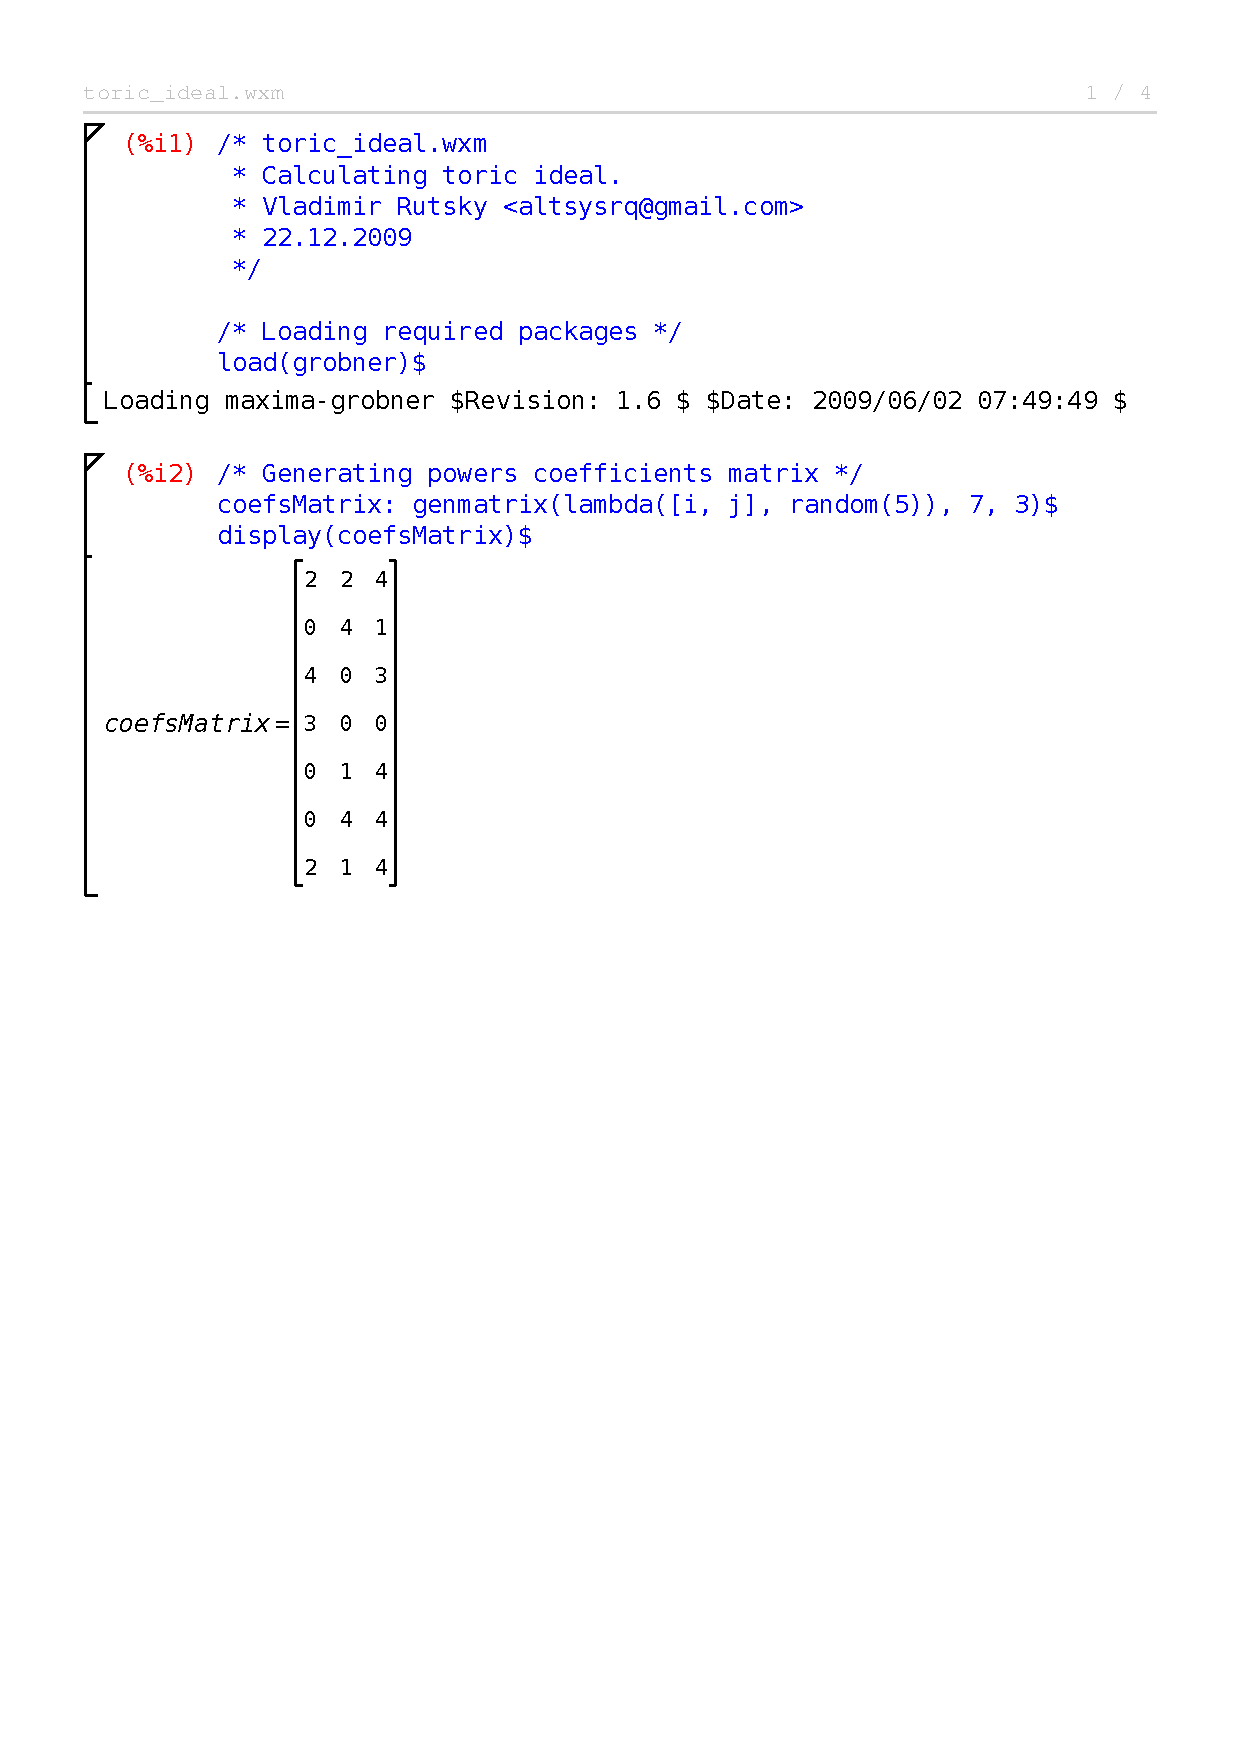
\includepdf[pages=-]{data/toric_ideal.pdf}

\end{document}
